  \let\negmedspace\undefined
\let\negthickspace\undefined
\documentclass[journal]{IEEEtran}
\usepackage[a5paper, margin=10mm, onecolumn]{geometry}
\usepackage{lmodern} % Ensure lmodern is loaded for pdflatex
\usepackage{tfrupee} % Include tfrupee package

\setlength{\headheight}{1cm} % Set the height of the header box
\setlength{\headsep}{0mm}     % Set the distance between the header box and the top of the text

\usepackage{gvv-book}
\usepackage{gvv}
\usepackage{cite}
\usepackage{amsmath,amssymb,amsfonts,amsthm}
\usepackage{algorithmic}
\usepackage{graphicx}
\usepackage{textcomp}
\usepackage{xcolor}
\usepackage{txfonts}
\usepackage{listings}
\usepackage{enumitem}
\usepackage{mathtools}
\usepackage{gensymb}
\usepackage{comment}
\usepackage[breaklinks=true]{hyperref}
\usepackage{tkz-euclide} 
\usepackage{listings}                                      
\def\inputGnumericTable{}                                 
\usepackage[latin1]{inputenc}                                
\usepackage{color}                                            
\usepackage{array}                                            
\usepackage{longtable}
\usepackage{multicol}
\usepackage{calc}                                             
\usepackage{multirow}                                         
\usepackage{hhline}                                           
\usepackage{ifthen}                                           
\usepackage{lscape}
\begin{document}
	
	\bibliographystyle{IEEEtran}
	\vspace{3cm}
	
	\title{11.16.3.3.4}
	\author{EE24BTECH11063 - Y. Harsha Vardhan Reddy }
	% \maketitle
	% \newpage
	% \bigskip
	{\let\newpage\relax\maketitle}
	
	\renewcommand{\thefigure}{\theenumi}
	\renewcommand{\thetable}{\theenumi}
	\setlength{\intextsep}{10pt} % Space between text and floats
	
	
	\numberwithin{equation}{enumi}
	\numberwithin{figure}{enumi}
	\renewcommand{\thetable}{\theenumi}
	
	
\textbf{Question}:\\
A die is rolled, Find the probability that a number greater than 6 will appear \\
\textbf{Solution: }\\
\textbf{Textual solution: }\\
Probability of a given event 'A'(A: Outcome is greater than 6),\\
\begin{align}
    \text{P(A)}=\frac{0}{6}=0
\end{align}
\textbf{Computational solution: }\\

\section*{Computation of Probabilities for Rolling a Die}

To compute the probability of obtaining specific outcomes when rolling a six-sided die, we rely on two key concepts: the **Probability Mass Function (PMF)** and the **Cumulative Distribution Function (CDF)**.

\subsection*{Definitions}
\subsubsection*{Probability Mass Function (PMF)}
The PMF represents the probability of each individual outcome in the sample space \( S \). For a six-sided die:
\[
S = \{1, 2, 3, 4, 5, 6\},
\]
the PMF is given as:
\[
P(X = x) = 
\begin{cases} 
\frac{1}{6}, & x \in S, \\ 
0, & x \notin S.
\end{cases}
\]

\subsubsection*{Cumulative Distribution Function (CDF)}
The CDF represents the cumulative probability of outcomes up to a given value \( x \), defined as:
\[
F(x) = P(X \leq x) = \sum_{k=1}^{x} P(X = k).
\]
For a six-sided die:
\[
F(x) = 
\begin{cases} 
0, & x < 1, \\
\frac{x}{6}, & x \in \{1, 2, 3, 4, 5, 6\}, \\
1, & x > 6.
\end{cases}
\]

\subsection*{Simulation Process}
We simulate the rolling of a die using the following steps:
\begin{enumerate}
    \item A six-sided die produces outcomes in the set:
    \[
    S = \{1, 2, 3, 4, 5, 6\}.
    \]
    \item For each simulated roll, a random integer \( X \) is generated such that \( X \in S \), using a random number generator function:
    \[
    X = (\text{rand()} \mod 6) + 1.
    \]
    \item The number of occurrences of each outcome is tracked over \( N \) trials, where \( N \) is the total number of simulations.
    \item Both the PMF and CDF are computed:
    \begin{itemize}
        \item **PMF**: The frequency of each outcome is divided by the total trials to compute the probability of each face.
        \item **CDF**: The cumulative probabilities are calculated as the running total of the PMF values.
    \end{itemize}
\end{enumerate}

\subsection*{Calculation of Probabilities}
\subsubsection*{Probability of Each Outcome (PMF)}
The probability of rolling each face \( i \) (\( i \in \{1, 2, 3, 4, 5, 6\} \)) is computed as:
\[
P(i) = \frac{\text{Number of rolls resulting in } i}{N}.
\]

\subsubsection*{Cumulative Probability (CDF)}
The cumulative probability up to face \( i \) is:
\[
F(i) = \sum_{k=1}^{i} P(k).
\]

\subsubsection*{Probability of Rolling \( X > 6 \)}
The probability of rolling a number greater than 6 is:
\[
P(X > 6) = \frac{\text{Number of rolls resulting in } X > 6}{N}.
\]
For a standard six-sided die, \( P(X > 6) = 0 \).

\subsection*{Output Representation}
The computed probabilities are represented in two forms:
\begin{itemize}
    \item **PMF**: The probabilities of rolling each face \( \{1, 2, 3, 4, 5, 6\} \), as well as the probability of \( X > 6 \).
    \item **CDF**: The cumulative probabilities up to each face, \( \{1, 2, 3, 4, 5, 6\} \), showing the cumulative likelihood of outcomes.
\end{itemize}
	\begin{figure}[h!]
		\centering
		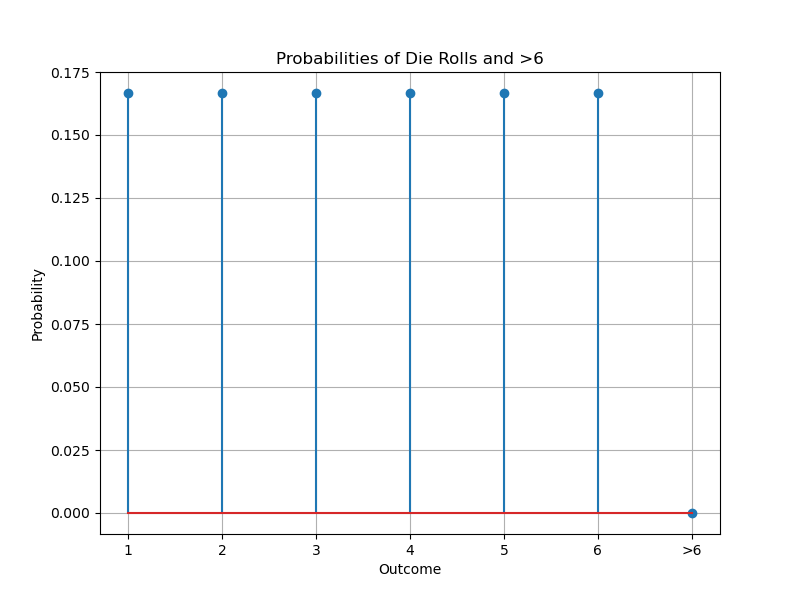
\includegraphics[width=\columnwidth]{figs/fig1.png}
		\caption{Solution of the system of linear equations}
		\label{stemplot}
	\end{figure}
	
\end{document}  
